\documentclass[conference]{IEEEtran}
\IEEEoverridecommandlockouts
\usepackage{cite}
\usepackage{amsmath,amssymb,amsfonts}
\usepackage{booktabs}
\usepackage{enumitem}
\usepackage{tikz}
\usetikzlibrary{arrows.meta,positioning}

\newcommand{\sat}{\operatorname{sat}}
\newcommand{\diag}{\operatorname{diag}}

\begin{document}

\title{Quanser QCar Autonomous Vehicle:\\ Hardware Physics, Identification, Modelling, and the Complete Controller Suite\\
{\footnotesize Mathematical foundations for offline simulation, digital-twin, and hardware execution}}

\author{\IEEEauthorblockN{Gandhi Contreras}
\IEEEauthorblockA{\textit{Electrical and Computer Engineering}, New Mexico State University, Las Cruces, NM, USA \\ gandhico@nmsu.edu}}

\maketitle

\begin{abstract}
The QCar is a 1/10-scale Ackermann-steered autonomous vehicle. This paper develops its complete control mathematics: the battery--drive--steering power chain, the drivetrain electromechanics through gear reduction to wheel force, tire--road interaction from the kinematic regime to linear cornering stiffness, the sensor suite physics (drive encoder, IMU, cameras, LiDAR) with the vision-based lane-error measurement model, identification experiments linear in the parameters, the kinematic and dynamic bicycle models with their lane-keeping error dynamics, and the full controller suite --- longitudinal PID, lateral PID, LQR, LQG, backstepping, sliding-mode, and NMPC --- including the implemented steering-envelope safety bounds.
\end{abstract}

\begin{IEEEkeywords}
QCar, Ackermann steering, bicycle model, lane keeping, cornering stiffness, LQR, LQG, backstepping, SMC, NMPC.
\end{IEEEkeywords}

%====================================================================
\section{Introduction}
The QCar couples a drive motor through a gearbox and differential to the rear axle, and a servo-actuated Ackermann front-steering linkage; perception (cameras, LiDAR, IMU) and computation ride on board. States of interest are the planar pose and velocity $(X, Y, \psi, v)$ and, for lane keeping, the error pair $x_e = [e_y,\ e_\psi]^{\!\top}$ (lateral offset and heading error to the path). Inputs are the normalized throttle $u_t$ and steering angle $\delta$, $|\delta|\le\delta_{\max} = 0.35$~rad --- the implemented steering envelope of our campaigns.

%====================================================================
\section{Hardware Physics}

\begin{figure*}[!t]
\centering
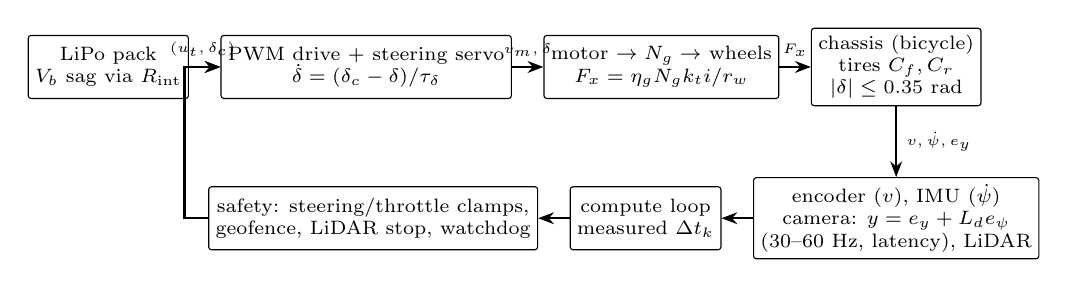
\begin{tikzpicture}[
  node distance=3mm and 4mm,
  blk/.style={draw, rounded corners=1pt, align=center, font=\scriptsize, inner sep=2.5pt, minimum height=8mm},
  lbl/.style={font=\tiny, align=center},
  arr/.style={-{Stealth[length=2mm]}, thick}
]

\node[blk] (bat) {LiPo pack\\ $V_b$ sag via $R_{\mathrm{int}}$};
\node[blk, right=of bat] (drv) {PWM drive + steering servo\\ $\dot\delta = (\delta_c - \delta)/\tau_\delta$};
\node[blk, right=of drv] (dtn) {motor $\to N_g \to$ wheels\\ $F_x = \eta_g N_g k_t i / r_w$};
\node[blk, right=of dtn] (veh) {chassis (bicycle)\\ tires $C_f, C_r$\\ $|\delta|\le0.35$ rad};
\node[blk, below=9mm of veh] (sens) {encoder ($v$), IMU ($\dot\psi$)\\ camera: $y = e_y + L_d e_\psi$\\ (30--60 Hz, latency), LiDAR};
\node[blk, left=of sens] (cmp) {compute loop\\ measured $\Delta t_k$};
\node[blk, left=of cmp] (safe) {safety: steering/throttle clamps,\\ geofence, LiDAR stop, watchdog};
\draw[arr] (bat) -- (drv);
\draw[arr] (drv) -- node[lbl, above] {$v_m,\delta$} (dtn);
\draw[arr] (dtn) -- node[lbl, above] {$F_x$} (veh);
\draw[arr] (veh) -- node[lbl, right] {$v,\dot\psi,e_y$} (sens);
\draw[arr] (sens) -- (cmp);
\draw[arr] (cmp) -- (safe);
\draw[arr] (safe.west) -- ++(-3mm,0) |- node[lbl, pos=0.75, above] {$(u_t,\delta_c)$} (drv.west);
\end{tikzpicture}
\caption{QCar signal chain: drivetrain and steering-servo lags, look-ahead vision measurement with camera latency, and the implemented $0.35$~rad steering envelope.}
\label{fig:chain}
\end{figure*}
\subsection{Power and drivetrain}
A LiPo pack ($V_b = v_{\mathrm{oc}}(\mathrm{SoC}) - R_{\mathrm{int}} i_b$ per cell) feeds a PWM drive stage; the averaged motor terminal voltage is $v_m = u_t V_b$. Manual-verified (QCar~2): 3S LiPo, nominal $11.1$~V, $3300$~mAh, $31$C discharge rating; firmware low-battery warning at $10.5$~V and automatic shutdown at $10.0$~V --- the undervoltage element of the safety envelope. The drive motor obeys $L_a\dot i + R_m i + k_e\omega_m = v_m$, $\tau_m = k_t i$; through the reduction $N_g$ (efficiency $\eta_g$) and wheel radius $r_w$, the tractive force and vehicle-speed coupling are
\begin{equation}
F_x = \frac{\eta_g N_g}{r_w}\,k_t\,i,
\qquad
\omega_m = \frac{N_g}{r_w}\,v ,
\end{equation}
so at the vehicle level, with the fast electrical pole eliminated,
\begin{equation}
m_e\dot v = \frac{\eta_g N_g k_t}{r_w R_m}\Bigl(u_t V_b - \frac{k_e N_g}{r_w}v\Bigr) - F_{\mathrm{roll}} - F_{\mathrm{drag}},
\label{eq:longit}
\end{equation}
where $m_e = m + J_{\mathrm{dt}}N_g^2/r_w^2$ is the drivetrain-augmented mass, $F_{\mathrm{roll}} = c_{rr} m g$, $F_{\mathrm{drag}} = \tfrac12\rho C_d A v^2$ (small at scale). Equation \eqref{eq:longit} is first order in $v$: gain and time constant are the two longitudinal identification targets. The steering servo is an internally position-controlled actuator: $\dot\delta = (\delta_c - \delta)/\tau_\delta$ with rate/angle limits --- a first-order lag that matters at lane-keeping bandwidth.

\subsection{Tires}
In the kinematic regime (low lateral acceleration) wheels roll without slip. Beyond it, each axle develops lateral force linear in slip angle, $F_{y,f} = -C_f\,\alpha_f$, $F_{y,r} = -C_r\,\alpha_r$, with slip angles
\begin{equation}
\alpha_f = \beta + \frac{l_f\dot\psi}{v} - \delta,\qquad
\alpha_r = \beta - \frac{l_r\dot\psi}{v},
\end{equation}
$\beta$ the sideslip; cornering stiffnesses $(C_f, C_r)$ are tire-physics parameters (carcass deformation) identified in E3 below. Saturation of the linear tire law bounds the validity region ($|\alpha| \lesssim 5^\circ$ at scale).

\subsection{Sensors}
Drive-shaft quadrature encoder ($720$ counts/rev pre-gearing on the QCar~2; speed via $v = r_w\omega_m/N_g$, quantization-limited at low speed hence filtered differentiation); MEMS IMU (gyro bias/noise as in our other platforms; yaw rate $\dot\psi$ feedback); CSI cameras and depth camera for the lane measurement; 2-D LiDAR for obstacles (QCar~2 suite: four CSI cameras, Intel RealSense RGB-D, RPLIDAR A2M12, NVIDIA Jetson AGX Orin compute). The \emph{vision measurement model} for lane keeping: a camera at look-ahead $L_d$ reports
\begin{equation}
y_{\mathrm{cam}} = e_y + L_d\,e_\psi + n_{\mathrm{cam}},
\label{eq:vision}
\end{equation}
the classical look-ahead output whose zero location $-1/L_d$ (in the error dynamics) is what makes moderate $L_d$ stabilizing --- the physical reason look-ahead distance is a design parameter, not an implementation detail. Frame latency (30--60~Hz camera vs.\ 100--500~Hz control) enters as an output delay in the lateral loop.

\subsection{Loop and safety}
Sampled loop with ZOH and measured-$\Delta t$ discipline as on all our platforms; safety envelope: $|\delta|\le0.35$~rad, throttle bound and low-speed torque clamp, geofence/lane-departure stop, watchdog on camera staleness, undervoltage lockout, and remote kill.

%====================================================================
\section{Vehicle Models}
\subsection{Kinematic bicycle}
Collapsing each axle to a single wheel (wheelbase $L = l_f + l_r$),
\begin{equation}
\dot X = v\cos\psi,\quad
\dot Y = v\sin\psi,\quad
\dot\psi = \frac{v}{L}\tan\delta,
\label{eq:kinbike}
\end{equation}
valid when tire slip is negligible; with \eqref{eq:longit} it is the complete low-speed model and the digital-twin default.

\subsection{Dynamic bicycle (linear tires)}
At speed, lateral dynamics in $(\beta, \dot\psi)$ or $(v_y,\dot\psi)$:
\begin{equation}
\begin{bmatrix}\dot v_y\\ \ddot\psi\end{bmatrix} =
\begin{bmatrix}
-\frac{C_f+C_r}{m v} & -v + \frac{C_r l_r - C_f l_f}{m v}\\[3pt]
\frac{C_r l_r - C_f l_f}{I_z v} & -\frac{C_f l_f^2 + C_r l_r^2}{I_z v}
\end{bmatrix}
\begin{bmatrix}v_y\\ \dot\psi\end{bmatrix}
+
\begin{bmatrix}\frac{C_f}{m}\\[2pt] \frac{C_f l_f}{I_z}\end{bmatrix}\delta,
\label{eq:dynbike}
\end{equation}
speed-parameterized ($v$ enters the matrices), with understeer gradient $K_{us} = \frac{m}{L}\bigl(\frac{l_r}{C_f} - \frac{l_f}{C_r}\bigr)$ summarizing the steady-state steering physics.

\subsection{Lane-keeping error dynamics}
Relative to a path of curvature $\kappa(s)$,
\begin{equation}
\dot e_y = v\sin e_\psi \approx v\,e_\psi,
\qquad
\dot e_\psi = \frac{v}{L}\tan\delta - v\,\kappa \approx \frac{v}{L}\delta - v\kappa,
\label{eq:laneerr}
\end{equation}
in the kinematic regime (the dynamic version substitutes \eqref{eq:dynbike}); $v\kappa$ is the measurable disturbance feedforward. This two-state model with the look-ahead output \eqref{eq:vision} and the servo lag is the lateral design plant; our campaign's implemented steering baseline is a stabilizing static gain on $[e_y,\ e_\psi]$ with the $0.35$~rad envelope.

%====================================================================
\section{Identification}

\begin{figure}[!t]
\centering
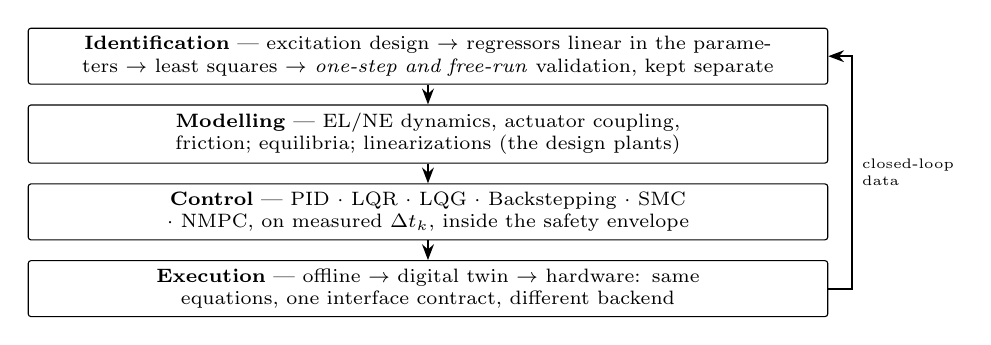
\begin{tikzpicture}[
  node distance=2.5mm,
  blk/.style={draw, rounded corners=1pt, align=center, font=\scriptsize, inner sep=3pt, text width=0.82\columnwidth},
  arr/.style={-{Stealth[length=2mm]}, thick}
]
\node[blk] (id) {\textbf{Identification} --- excitation design $\to$ regressors linear in the parameters $\to$ least squares $\to$ \emph{one-step and free-run} validation, kept separate};
\node[blk, below=of id] (mod) {\textbf{Modelling} --- EL/NE dynamics, actuator coupling, friction; equilibria; linearizations (the design plants)};
\node[blk, below=of mod] (ctl) {\textbf{Control} --- PID $\cdot$ LQR $\cdot$ LQG $\cdot$ Backstepping $\cdot$ SMC $\cdot$ NMPC, on measured $\Delta t_k$, inside the safety envelope};
\node[blk, below=of ctl] (exe) {\textbf{Execution} --- offline $\to$ digital twin $\to$ hardware: same equations, one interface contract, different backend};
\draw[arr] (id) -- (mod);
\draw[arr] (mod) -- (ctl);
\draw[arr] (ctl) -- (exe);
\draw[arr] (exe.east) -- ++(3mm,0) |- node[font=\tiny, pos=0.25, right, align=left] {closed-loop\\ data} (id.east);
\end{tikzpicture}
\caption{The workflow every platform in this series follows: identification feeds modelling, modelling feeds the controller suite, and all stages run unchanged across the three execution targets; closed-loop records return to identification.}
\label{fig:workflow}
\end{figure}
\begin{enumerate}[label=E\arabic*)]
\item \emph{Longitudinal}: throttle steps/PRBS at several $V_b$; fit gain and time constant of \eqref{eq:longit} (linear least squares on $\dot v = a v + b u_t + c$); coast-down runs separate $c_{rr}$ and drag.
\item \emph{Steering servo}: $\delta_c$ steps against IMU yaw rate at constant speed via \eqref{eq:kinbike}: extract $\tau_\delta$ and the effective steering gain (linkage compliance shows up here).
\item \emph{Cornering stiffness}: constant-speed steering chirps; regress \eqref{eq:dynbike} --- linear in $(C_f, C_r)$ given $(m, I_z, l_f, l_r)$; $I_z$ from a trifilar pendulum swing of the chassis, $l_f, l_r$ from wheel scales.
\item \emph{Validation}: held-out records, one-step and free-run fits reported separately; free-run of \eqref{eq:laneerr} closed against logged steering reproduces the lane trace within the linear-tire envelope.
\end{enumerate}

%====================================================================
\section{Control Suite}
Longitudinal and lateral loops are designed separately (bandwidth-decoupled) with the suite applied to the lateral plant \eqref{eq:laneerr}--\eqref{eq:dynbike}; all discrete updates use measured $\Delta t_k$; steering commands clip at $0.35$~rad.

\subsection{PID}
Longitudinal cruise: PI on speed error with anti-windup against the throttle bound, plus the $V_b$ gain schedule. Lateral: PD on the look-ahead output \eqref{eq:vision},
$\delta = -k_p\,y_{\mathrm{cam}} - k_d\,\dot y_{\mathrm{cam}} + L\kappa$ (curvature feedforward), the derivative from the shared second-order filter.

\subsection{LQR / LQG}
On $x_\ell = [e_y,\ e_\psi,\ \delta]^{\!\top}$ (servo lag appended) or the four-state dynamic version, $\delta_c = -K_{\mathrm{lqr}}x_\ell + k_{\mathrm{ff}}\kappa$ with the CARE gain; because \eqref{eq:dynbike} is speed-varying, $K_{\mathrm{lqr}}(v)$ is gain-scheduled on measured speed. LQG closes the loop from the vision output \eqref{eq:vision} alone: the Kalman filter reconstructs $(e_y, e_\psi)$ through the look-ahead mixing and the camera delay, with measurement covariance from lane-detector residuals.

\subsection{Backstepping}
Strict-feedback chain $e_y \to e_\psi \to \delta$: with $z_1 = e_y$, virtual heading $e_\psi^d = -c_1 z_1/v$; $z_2 = e_\psi - e_\psi^d$; virtual steering from \eqref{eq:laneerr}; $z_3 = \delta - \delta^d$ through the servo lag. The composite $V = \tfrac12(z_1^2 + z_2^2 + z_3^2)$ yields $\dot V = -\sum c_i z_i^2$ with the final command $\delta_c = \tau_\delta\bigl(\dot\delta^d - z_2\,\partial(\cdot) - c_3 z_3\bigr) + \delta$ --- the systematic way the servo lag is absorbed rather than ignored.

\subsection{Sliding mode}
$s = \dot e_y + \lambda e_y = v e_\psi + \lambda e_y$;
$\delta = \delta_{\mathrm{eq}} - \eta\,\sat(s/\phi)$ with $\delta_{\mathrm{eq}}$ from \eqref{eq:laneerr} ($\dot s = 0$) including the curvature term; robustness margin $\eta$ sized against tire-stiffness and speed-estimate error; boundary layer $\phi$ set above the vision noise floor mapped through \eqref{eq:vision} to avoid noise-driven chatter.

\subsection{NMPC}
Receding horizon on the kinematic or dynamic bicycle with path preview:
\begin{align}
\min_{\{\delta_k, u_{t,k}\}}\ \sum_{k=0}^{N-1}& \Bigl( q_y e_{y,k}^2 + q_\psi e_{\psi,k}^2 + q_v (v_k - v_r)^2 \nonumber\\
&+ r_\delta \Delta\delta_k^2 + r_t \Delta u_{t,k}^2 \Bigr) + V_f
\end{align}
subject to \eqref{eq:kinbike}/\eqref{eq:dynbike} (RK4), $|\delta|\le0.35$, actuator rate limits, and the linear-tire validity constraint $|\alpha_{f,r}|\le\bar\alpha$ --- the constraint that makes NMPC the natural home for aggressive maneuvers; preview of $\kappa(s)$ over the horizon is the mathematical form of ``looking through the corner.'' Real-time reductions as on our other platforms (short horizon, move blocking, warm start).

%====================================================================
\section{Execution Modes and Conclusion}
Offline: \eqref{eq:longit}, \eqref{eq:kinbike}--\eqref{eq:laneerr} with sensor/latency models injectable. Digital twin: the vendor virtual QCar exposes the same actuation/measurement contract, including camera-based lane detection. Hardware: the physical car under the safety envelope. The mathematics above --- battery-to-tire-force physics, vision measurement geometry, speed-scheduled models linear in their identifiable parameters, and the six-controller lateral/longitudinal suite --- are common to all three targets and constitute the platform's single source of truth.

\bibliographystyle{IEEEtran}
\begin{thebibliography}{9}
\bibitem{rajamani2012} R.~Rajamani, \emph{Vehicle Dynamics and Control}, 2nd ed. Springer, 2012.
\bibitem{kong2015} J.~Kong, M.~Pfeiffer, G.~Schildbach, and F.~Borrelli, ``Kinematic and dynamic vehicle models for autonomous driving control design,'' \emph{IEEE IV}, 2015.
\bibitem{pacejka2012} H.~Pacejka, \emph{Tire and Vehicle Dynamics}, 3rd ed. Butterworth-Heinemann, 2012.
\bibitem{quanser_qcar} Quanser Consulting Inc., \emph{QCar User Manual}, Markham, ON, Canada.
\bibitem{khalil2002} H.~K. Khalil, \emph{Nonlinear Systems}, 3rd ed. Prentice Hall, 2002.
\bibitem{utkin1992} V.~Utkin, \emph{Sliding Modes in Control and Optimization}. Springer, 1992.
\bibitem{rawlings2017} J.~B. Rawlings, D.~Q. Mayne, and M.~Diehl, \emph{Model Predictive Control}, 2nd ed. Nob Hill, 2017.
\bibitem{ljung1999} L.~Ljung, \emph{System Identification: Theory for the User}, 2nd ed. Prentice Hall, 1999.
\end{thebibliography}

\end{document}
